% =========================================================================
%  Philosophy of Intimacy and the Theory of Justice
%  VOLUME II — Papers X–XVIII
%  (generated by gen_volumes.py from the Volume I template)
% =========================================================================
\documentclass[11pt,twoside,openright]{book}

\usepackage{serendip-book}
\usepackage{pdfpages}
\usepackage{import}

\usepackage[backend=biber, style=authoryear, sorting=nyt,
            maxcitenames=2, uniquelist=false]{biblatex}
\addbibresource{../bib/master.bib}

\graphicspath{%
  {../papers/paper_10_joint_attention_of_value/}%
  {../papers/paper_11_just_eudaimonia/}%
  {../papers/paper_12_the_sweet_cycle/}%
  {../papers/paper_13_non_binding_vow/}%
  {../papers/paper_14_existentialist_eudaimonism/}%
  {../papers/paper_15_generative_relational_wealth/}%
  {../papers/paper_16_semiotics_of_luxury/}%
  {../papers/paper_17_generativity_under_power/}%
  {../papers/paper_18_generative_effacement/}%
}

\newcommand{\paperchapter}[3]{%
  \chapter{#2}%
  \ifx\relax#3\relax\else
    {\Large\itshape\color{warnred}#3\par}\vspace{1.4em}%
  \fi
  \clearpage           % chapter title page; abstract begins on its own page
  \begin{refsection}
    % normal section numbering per chapter (undo any previous paper's \appendix)
    \setcounter{section}{0}%
    \renewcommand{\thesection}{\thechapter.\arabic{section}}%
    \subimport{../papers/#1/}{content.tex}
    \printbibliography[heading=subbibliography, title={References}]
  \end{refsection}
}

\begin{document}

\frontmatter

% Designed front cover (VOLUME 2; author retained; SCS removed).
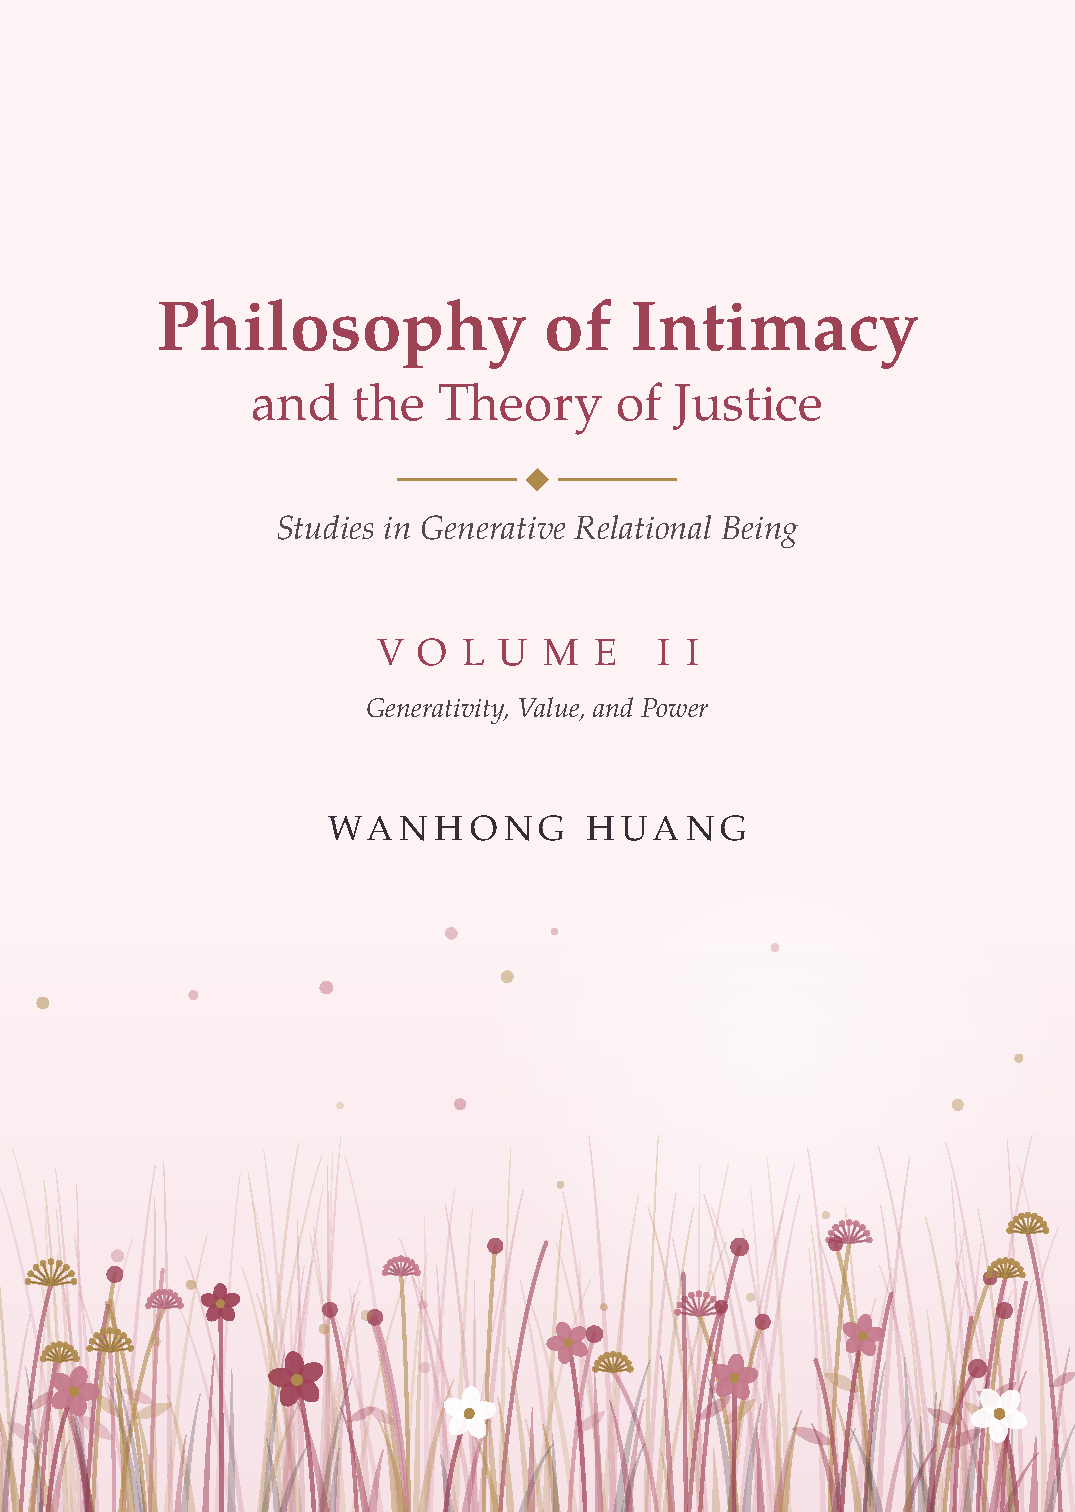
\includepdf[fitpaper=true,pages=1]{../assets/cover_front_vol2.pdf}

\import{../}{foreword.tex}

\tableofcontents

\mainmatter

\paperchapter{paper_10_joint_attention_of_value}
  {The Joint Attention of Value and the Creation of Language}
  {\relax}
\paperchapter{paper_11_just_eudaimonia}
  {A Just Eudaimonia}
  {\relax}
\paperchapter{paper_12_the_sweet_cycle}
  {The Sweet Cycle}
  {\relax}
\paperchapter{paper_13_non_binding_vow}
  {The Causality of the Non-Binding Vow}
  {On Trust, Promise, and the Generation of Expectation in the Absence of the Other's Sword}
\paperchapter{paper_14_existentialist_eudaimonism}
  {Contingency, Existence, and Eudaimonia in Intimate Relations}
  {\relax}
\paperchapter{paper_15_generative_relational_wealth}
  {The Political Economy of Intimate Relations}
  {Toward a Theory of Generative Relational Wealth}
\paperchapter{paper_16_semiotics_of_luxury}
  {The Semiotics of Luxury in Intimate Relations}
  {\relax}
\paperchapter{paper_17_generativity_under_power}
  {Generativity Under Power}
  {\relax}
\paperchapter{paper_18_generative_effacement}
  {Generative Effacement in the Intimate Relation}
  {\relax}

\backmatter

% Designed back cover (SCS removed).
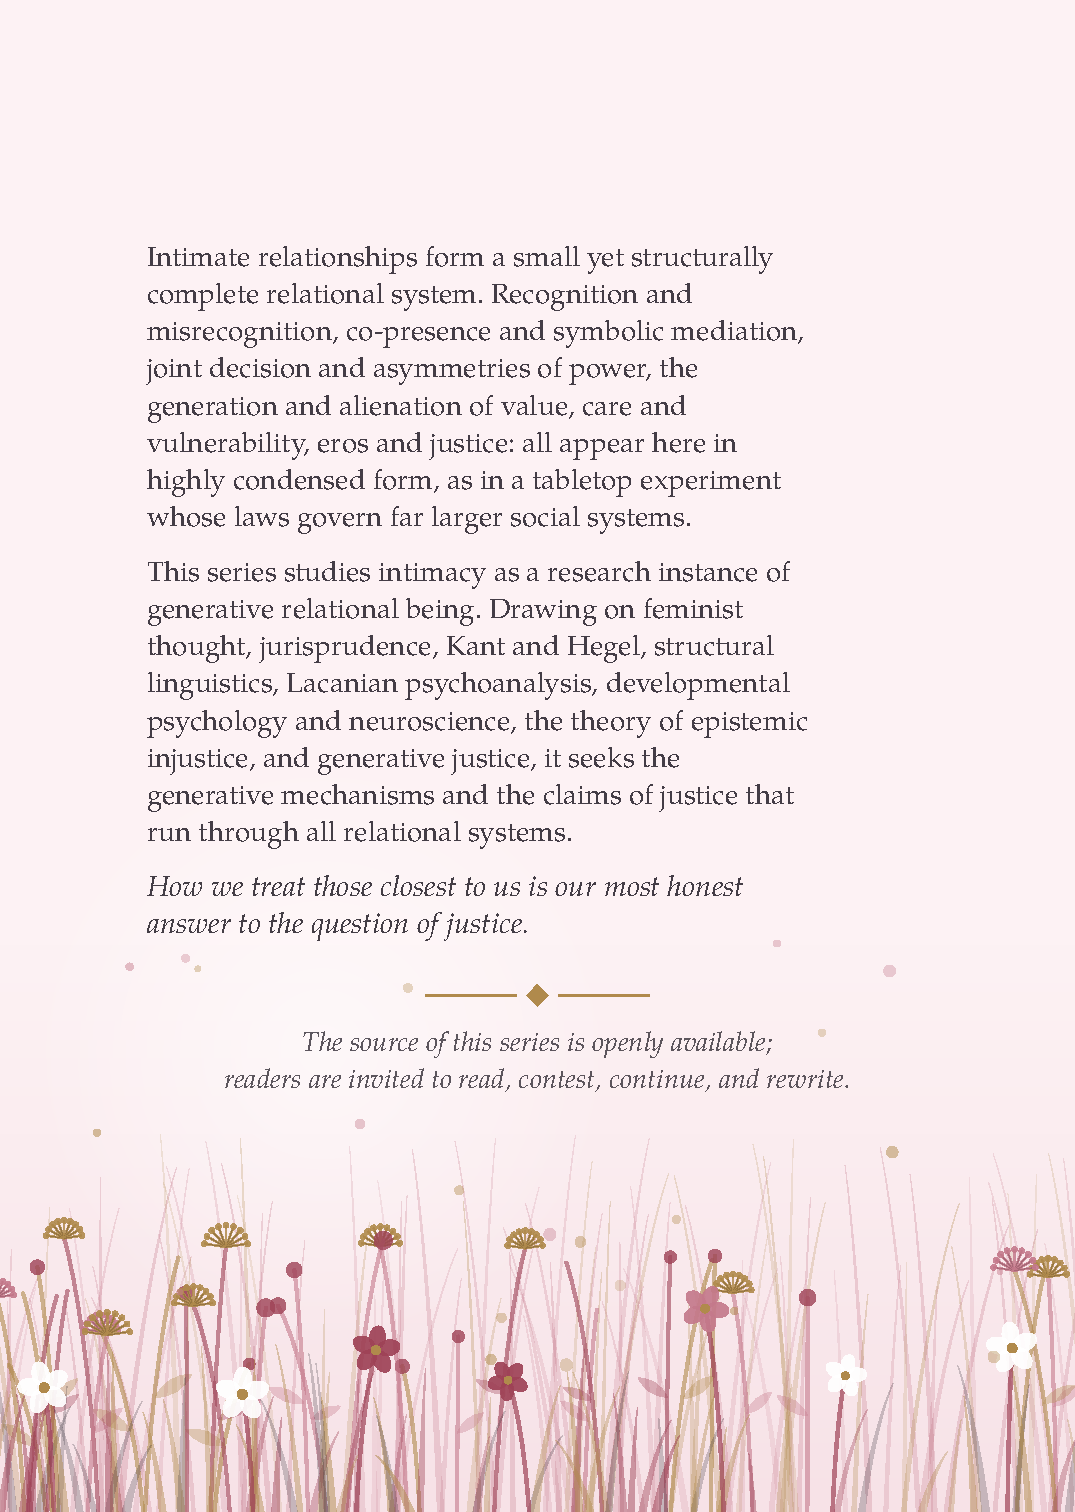
\includepdf[fitpaper=true,pages=1]{../assets/cover_back_book.pdf}

\end{document}
